\documentclass[10pt,svgnames,usenames,table]{beamer} %,handout si version papier
\NeedsTeXFormat{LaTeX2e} 

\usetheme[compress]{Singapore} % theme

\usepackage[french]{babel}
\usepackage[utf8x]{inputenc} % pour les accents (mettre latin1 pour
                            % windows au lieu de utf8)
\usepackage[T1]{fontenc}
\usepackage{amsmath,amsthm,amssymb}        % un packages mathématiques
\usepackage{xcolor}         % pour définir plus de couleurs
\usepackage{graphicx}       % pour insérer des figures
\usepackage{lmodern}
\usepackage{url}
	\urlstyle{sf}
\usepackage{lastpage}
\usepackage{endnotes}
\usepackage{listings}
\usepackage[french]{varioref}
\usepackage{wrapfig}
\usepackage{pdfpages}
\usepackage{verbatim}
\usepackage{graphicx}

%\usepackage[svgnames]{color}
%\definecolor{webdarkblue}{rgb}{0,0,0.4}
%\definecolor{webgreen}{rgb}{0,0.3,0}
%\definecolor{webblue}{rgb}{0,0,0.8}

\setbeamercolor{section in head/foot}{use=structure,bg=structure.fg!25!bg} % "Amélioration du jeu de couleur"
%\useoutertheme[subsection=true]{smoothbars} % Pour avoir un rappel de la subsection
\setbeamerfont{frametitle}{series=\bfseries}
\setbeamertemplate{frametitle}[default][center] % Titre centré et bien placé.


% "Fioriture de style" : qd <x-> dans les item, les autres en gris clair
\beamertemplatetransparentcovered


% Comportement des itemize
\setbeamertemplate{itemize item}[ball]
\setbeamertemplate{itemize subitem}[triangle]
\setbeamertemplate{itemize subsubitem}[circle]

%\renewcommand\sfdefault{cmss} % Polices

% Les block arrondis et ombrés dans la couleur que je veux
\setbeamertemplate{blocks}[rounded][shadow=true]
\definecolor{normalBlockColor}{RGB}{102,153,255}
\definecolor{normalTitleBlockColor}{RGB}{0,0,102}
\definecolor{normalBlockTextColor}{RGB}{255,255,255}
\definecolor{normalBlockTitleTextColor}{RGB}{255,255,255}
\definecolor{exampleBlockColor}{RGB}{202,251,197}
\definecolor{exampleTitleBlockColor}{RGB}{166,241,158}
\definecolor{exampleBlockTextColor}{RGB}{0,0,0}
\definecolor{exampleBlockTitleTextColor}{RGB}{0,120,0}
\definecolor{alertBlockColor}{RGB}{248,218,218}
\definecolor{alertTitleBlockColor}{RGB}{244,108,108}
\definecolor{alertBlockTextColor}{RGB}{0,0,0}
\definecolor{alertBlockTitleTextColor}{RGB}{120,0,0}
\setbeamercolor*{block title}{fg=normalBlockTitleTextColor,bg=normalTitleBlockColor}
\setbeamercolor*{block body}{fg=normalBlockTextColor,bg=normalBlockColor}
\setbeamercolor*{block title alerted}{fg=alertBlockTitleTextColor,bg=alertTitleBlockColor}
\setbeamercolor*{block body alerted}{fg=alertBlockTextColor,bg=alertBlockColor}
\setbeamercolor*{block title example}{fg=exampleBlockTitleTextColor,bg=exampleTitleBlockColor}
\setbeamercolor*{block body example}{fg=exampleBlockTextColor,bg=exampleBlockColor}
\setbeamerfont{block title}{size={}}



%------------ fin style beamer -------------------

% Faire apparaître un sommaire avant chaque section
% \AtBeginSection[]{
%   \begin{frame}
%   \frametitle{Plan}
%   \medskip
%   %%% affiche en début de chaque section, les noms de sections et
%   %%% noms de sous-sections de la section en cours.
%   \small \tableofcontents[currentsection, hideothersubsections]
%   \end{frame} 
% }


% Pour personnaliser la barre de navigation du dessous
\setbeamertemplate{navigation symbols}{
	%\insertslidenavigationsymbol
	%\insertframenavigationsymbol
	%\insertsubsectionnavigationsymbol
	\quad\textbf{\insertframenumber/\inserttotalframenumber} % Numéro de page
	%\insertsectionnavigationsymbol
	%\insertdocnavigationsymbol
	%\insertbackfindforwardnavigationsymbol
}
% Supprimer les icones de navigation (pour les transparents)
%\setbeamertemplate{navigation symbols}{}

% Mettre les icones de navigation en mode vertical (pour projection)
% \setbeamertemplate{navigation symbols}[vertical]

\newenvironment{itemize2}%
	{ \begin{list}%
		{$\bullet$}%
		{\setlength{\labelwidth}{30pt}%
		 \setlength{\leftmargin}{35pt}%
		 \setlength{\itemsep}{\parsep}}}%    
	{ \end{list} }

\def\siecle#1{\textsc{\romannumeral #1}\textsuperscript{e}~siècle} % => le \siecle{19}

\definecolor{codeBlue}{rgb}{0,0,1}
\definecolor{webred}{rgb}{0.5,0,0}
\definecolor{codeGreen}{rgb}{0,0.5,0}
\definecolor{codeGrey}{rgb}{0.6,0.6,0.6}
\definecolor{webdarkblue}{rgb}{0,0,0.4}
\definecolor{webgreen}{rgb}{0,0.3,0}
\definecolor{webblue}{rgb}{0,0,0.8}
\definecolor{orange}{rgb}{0.7,0.1,0.1}
\lstset{
      language=C,
      flexiblecolumns=true,
      numbers=left,
      stepnumber=1,
      numberstyle=\ttfamily\tiny,
      keywordstyle=\ttfamily\textcolor{blue},
      stringstyle=\ttfamily\textcolor{red},
      commentstyle=\ttfamily\textcolor{green},
      breaklines=true,
      extendedchars=true,
      basicstyle=\ttfamily\scriptsize,
      showstringspaces=false
    }

\usepackage{pdflscape} %% portrait
\usepackage[french]{varioref} % \vpageref

\graphicspath{{img/}}
\definecolor{gris}{RGB}{228,228,228}
\definecolor{bleu}{RGB}{34,148,255}
\definecolor{darkgray}{rgb}{0.3,0.3,0.3}


\logo{
\includegraphics[height=5mm]{logo_12-13-mini.png}}
\institute{Louvain-li-Nux}
\title{\textbf{Formation \LaTeX}\\Introduction à l'écriture de document \textrm{\LaTeX}}
\author{Arnaud \textsc{Cerckel} \and Benoît \textsc{Legat}}

\date{25 mars 2014}



\begin{document}

%%%%%%%%%%%% SIDA
\begin{landscape}
\begin{frame}[noframenumbering,plain]
	\vspace{-.5cm}
	\hspace*{.1mm}
	
\includegraphics[page=1,height=\paperwidth]{latex_sida.pdf}
\end{frame}
\end{landscape}
%%%%%%%%%%%%

\begin{frame}
\maketitle
Merci à Jolan \textsc{Wolter} et Thomas \textsc{Vanzieleghem} pour avoir réalisé la première version de ces slides
ainsi qu'à David \textsc{Ernst} et Matthieu \textsc{Baerts} pour avoir réalisé la deuxième version.
\end{frame}

\AtBeginSection[]
  {
     \begin{frame}<beamer>
     \frametitle{\insertsection}
     \tableofcontents[hideothersubsections]
     \end{frame}
  }

\section{Introduction}
\subsection{Qu'est-ce que \LaTeX{}?}
\begin{frame}
\frametitle{Qu'est ce que \LaTeX}

\begin{itemize}
\item \TeX{} $ \Rightarrow$ programme de mise en page
\vspace{0.5cm}
\item \LaTeX{} $ \Rightarrow$ ensemble de commanges qui seront
 interprétées par le programme \TeX
 \vspace{0.5cm}
\item \LaTeX{} $ \neq$ WYSIWYG (What You See Is What You Get)
\end{itemize}

\end{frame}

\subsection{Pourquoi \LaTeX{}?}
\begin{frame}{Pourquoi \LaTeX{}?}

  \begin{itemize}
  	\item Qualité professionnelle de document
	\item Facilité d'emploi des :
	\begin{itemize}
		\item formules mathématiques
		\item table des matières
		\item références bibliographiques
		\item références croisées
		\item ...
	\end{itemize}
	\item Ne se préoccuper que du contenu
	\item Forme $\neq$ esthétique
	\item Forme = message
	\item Gratuit
	\item Stable, même pour les très gros documents
  \end{itemize}
\end{frame}

\begin{frame}{Pourquoi \LaTeX{}?}

\begin{figure}[htbp]
\begin{center}
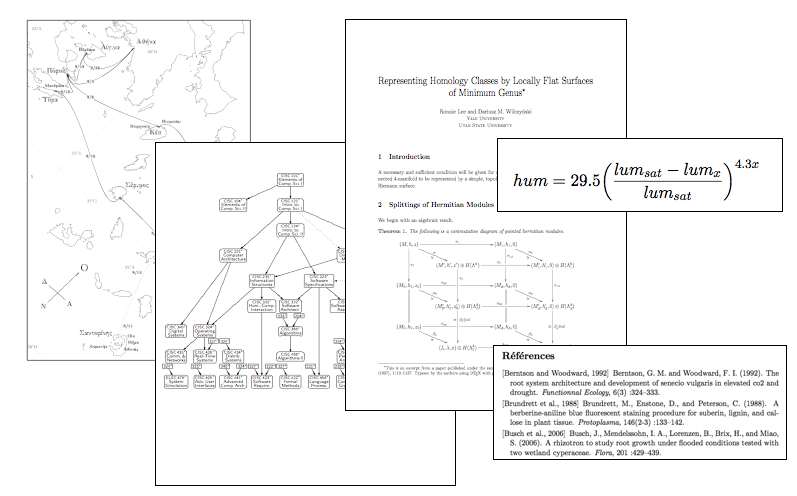
\includegraphics[height=6.5cm]{latex_exemples}
\end{center}
\end{figure}
\end{frame}

%-----------------------
\subsection{Pourquoi pas \LaTeX{}?}
\begin{frame}{Pourquoi pas \LaTeX{}?}

  \begin{itemize}
  	\item Les tableaux...
	\item Prise en main plus longue que pour traitement de texte WYSIWYG
	\item Je suis allergique à toute forme de code informatique
	\item J'ai des actions chez Microsoft Office
	\item Je ne trouve pas le "\textbackslash " sur mon clavier
  \end{itemize}
\end{frame}

%-----------------------
\subsection{Les Outils}
\begin{frame}{Ce qu'il faut pour commencer.}

  \begin{itemize}
	  \item GNU/Linux
	  \begin{itemize}
	  	\item Distribution \LaTeX{} = \textbf{TeXLive}
		\item Éditeur de texte = \textbf{TeXMaker, LaTeXila, Kile}
	  \end{itemize}
	  \item Windows
	  \begin{itemize}
	  	\item Distribution \LaTeX{} = \textbf{MikTeX}
		\item Éditeur de texte = \textbf{TeXMaker, TeXnicCenter}
	  \end{itemize}
	  \item Mac OS
	  \begin{itemize}
	  	\item Distribution \LaTeX{} = \textbf{MacTeX}
		\item Éditeur de texte =\textbf{TeXMaker, TeXShop, iTeXMac}
	  \end{itemize}
  \end{itemize}
\end{frame}

\section{Les concepts de base}
\subsection{Les fichiers}

\begin{frame}{Les fichiers}

	\begin{center}
		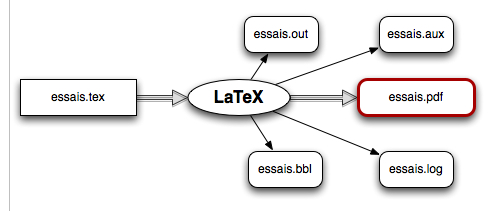
\includegraphics[height=3cm]{compilation.jpg}
	\end{center}

	\begin{itemize}
		\item Fichier source  = essai\alert{\textbf{.tex}}
		\item Lors de compilation $\rightarrow$ création de nombreux fichiers annexes
		\begin{itemize}
			\item style, class;
			\item structure du document;
			\item table des matières, liste des figures;
			\item liste des références;
			\item ...
		\end{itemize}
		\item Création d'un fichier essai\alert{\textbf{.pdf}}
	\end{itemize}
\end{frame}

%-----------------------
\subsection{La structure}

\begin{frame}[fragile]{Structure générale du document}
\framesubtitle{Séparation du préambule et du corps du document}
\small
\begin{columns}
	\begin{column}[b] {3.3cm}
		Type de document\\ 
		Utilisation de \textit{package}\\ 
		Utilisation de \textit{package}\\
		Utilisation de \textit{package}\\
		\vspace{0.3cm}
		%\hline
		\vspace{0.2cm}
		Début du document \\
		Corps du document  \\
		Fin du document \\ 
	\end{column}
	\begin{column}[b] {3cm}
		\begin{verbatim}
			\documentclass[a4paper, 10pt]{article}	
			\usepackage[latin1]{inputenc}
			\usepackage[T1]{fontenc}
			\usepackage[french]{babel}

			\begin{document}
			Ceci est mon premier document en \LaTeX{}
			\end{document}
		\end{verbatim}
	\end{column}
	\begin{column}[b] {3cm}
	\end{column}
\end{columns}


\end{frame}

%-----------------------

\subsection{Les classes}

\begin{frame}[fragile]{Les principales classes de document}
\begin{tabular}{lp{8cm}}
\textbf{article} & for articles in scientific journals, presentations, short reports, program documentation, invitations, ...\\
\textbf{report} & for longer reports containing several chapters, small books, thesis, ...\\
\textbf{book} & for real books.\\
\textbf{letter} & for writing letters.\\
\textbf{beamer} & for writing presentations.
\end{tabular}
\vspace{1cm}
\begin{center}
\verb|\documentclass[a4paper,10pt]{article}|\\
\end{center}
\end{frame}

\subsection{La structure}
\begin{frame}[fragile]{La structure logique du document}
	\begin{itemize}
		\item Structure logique du document uniquement
		\item \LaTeX{} se charge de la numérotation et de la mise en page\\
	\end{itemize}
	\vspace{1cm}
	
	\verb|\part{}|\\
	\hspace{1cm} \verb|\chapter{}| \hspace{2cm}$\Longrightarrow$ \textcolor{bleu}{uniquement \textit{books}}\\
	\hspace{2cm} \verb|\section{}|\\
	\hspace{3cm} \verb|\subsection{}| \\
	\hspace{4cm} \verb|\subsubsection{}| \\
	\hspace{5cm} \verb|\paragraph{}	| \\
	
\end{frame}

%-----------------------
\section{Mise en page générale}
\subsection{La table des matières}
\begin{frame}[fragile]{Table des matières}
	\begin{itemize}
		\item Une ligne de commande suffit pour générer toute la table des matières
	\end{itemize}
	\begin{columns}
	\column{0.5\textwidth}
	\vspace{0.3cm}
	\small
	\verb|\documentclass[a4paper,10pt]{article}|\\
	\verb|\usepackage[francais]{babel} |\\
	\verb|\usepackage[latin1]{inputenc}|\\
	\verb|\usepackage[T1]{fontenc}|\\
	\vspace{0.4cm}
	\verb|\begin{document} |\\
	{\usebeamercolor[fg]{example text} \verb|\tableofcontents|}\\
	\verb|\section{Section 1} |\\
	\verb|Ceci est mon premier document écrit en TEX |\\
	\verb|\section{Section 2} |\\
	\verb|Ceci est ma deuxième section |\\
	\verb|\subsection{Sous-section 2.1} |\\
	\verb|Ceci est une sous-section|\\
	\verb|\end{document}|
	\column{0.5\textwidth}
	\begin{flushright}
	\fbox{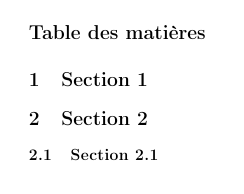
\includegraphics[width=0.6\textwidth]{table.png}}
	\end{flushright}
	\end{columns}
\end{frame}

%-----------------------
\subsection{La taille des polices}
\begin{frame}[fragile]{Jouer avec les fontes}
\framesubtitle{Changer la taille et le type de police}
	\begin{center}
	\fbox{
\includegraphics[width=0.7\textwidth]{font.png}}
	\end{center}
	\small
	\verb|\documentclass[a4paper,10pt]{article}|\\
	\verb|\usepackage[french]{babel} |\\
	\verb|\usepackage[T1]{fontenc}|\\
	\verb|\usepackage[latin1]{inputenc}|\\
	\vspace{0.4cm}
	\verb|\begin{document} |\\
	\verb|Ceci est mon premier document écrit en \LaTeX{} |\\
	{\usebeamercolor[fg]{example text} \verb|\huge|}\\
	\verb|Ecrit un peu plus grand. |\\
	{\usebeamercolor[fg]{example text} \verb|\sffamily |}\\
	\verb|Dans une autre police de caractère|\\
	\verb|\end{document}|

\end{frame}

\subsection{Mise en forme simple}
\begin{frame}[fragile]{Mise en forme simple}
\footnotesize 
\begin{lstlisting}[frame=single,language=TeX]
	Je peux mettre en \textbf{gras}, en \textit{italique}, en \texttt{machine a
	ecrire}, dans un format pour les \textsc{Noms}, etc. % c'est ecrit sur 2 lignes
	
	Voici un nouveau paragraphe.\\ % un commentaire

	Mais j'ai envie d'avoir une separation avec le reste du texte en ajoutant une ligne vide.\\
	(je peux aussi forcer le retour a la ligne, a vous de choisir le style).
\end{lstlisting}
\begin{center}
	\fbox{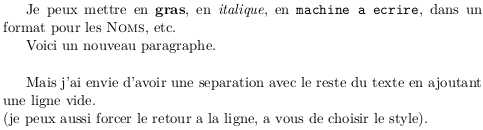
\includegraphics[width=\textwidth]{mise_en_page_simple.png}}
	\end{center}
\end{frame}

%-----------------------
\subsection{Les listes}
\begin{frame}[fragile]{Les listes}
	\begin{itemize} 
		\item Trois types de listes: \verb|itemize|, \verb|enumerate| et \verb|description|
	\end{itemize}
	\vspace{0.5cm}
	\hspace{1cm} \verb|\begin{|{\usebeamercolor[fg]{example text} \verb|itemize|}\verb|} |\\
	\hspace{2cm} \verb|\item Premier élément de la liste|\\ 
	\hspace{2cm} \verb|\item Deuxième élément de la liste|\\ 
	\hspace{1cm} \verb|\end{|{\usebeamercolor[fg]{example text} \verb|itemize|}\verb|} |\\
	\vspace{0.5cm}
	
	\fbox{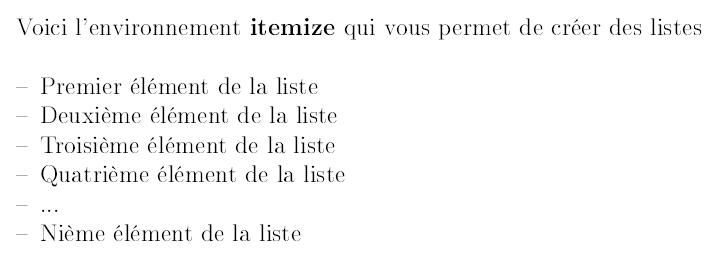
\includegraphics[width=\textwidth]{liste.jpg}}
\end{frame}

%-----------------------
\section{Les environnements flottants}
\subsection{Les figures}
\begin{frame}[fragile]{Les figures}
	\fbox{
\includegraphics[width=\textwidth]{figure.jpg}}
\end{frame}

\begin{frame}[fragile]{Les figures}
%\framesubtitle{Un contenant pour des éléments de type \textit{table} et \textit{figure}}

\begin{verbatim}
Sur la figure~\ref{ucl}, vous pouvez voir le logo UCL 
mis à 50 \% de la largueur du texte.

\begin{figure}[H]
    \centering
        
\includegraphics[width=0.50\textwidth]{logo-ucl.jpg}
    \caption{Voici le logo UCL}
    \label{ucl}
\end{figure}
\end{verbatim}
\end{frame}
%	\vspace{0.5cm}
%	\hspace{1cm} \verb|\begin{|{\usebeamercolor[fg]{example text} \verb|itemize|}\verb|} |\\
%	\hspace{2cm} \verb|\item Premier élément de la liste|\\ 
%	\hspace{2cm} \verb|\item Deuxième élément de la liste|\\ 
%	\hspace{1cm} \verb|\end{|{\usebeamercolor[fg]{example text} \verb|itemize|}\verb|} |\\
%	\vspace{0.5cm}

\subsection{Les tableaux}
\begin{frame}[fragile]{Les tableaux}
\begin{footnotesize}
\begin{verbatim}
\begin{table}[H]
    \begin{center}
            \begin {tabular}{|l||c|} %% 2 columns
            \hline
                \textit{Inventaire} & \textbf{Nombre} \\
            \hline
                Chemises  & 4   \\
                Pulls     & 12  \\
                Pantalons & 1   \\
            \hline
            \end{tabular}
        \caption{Tableau relatif à l'inventaire}
    \end{center}
\end{table}
\end{verbatim}
\end{footnotesize}
\begin{center}
\fbox{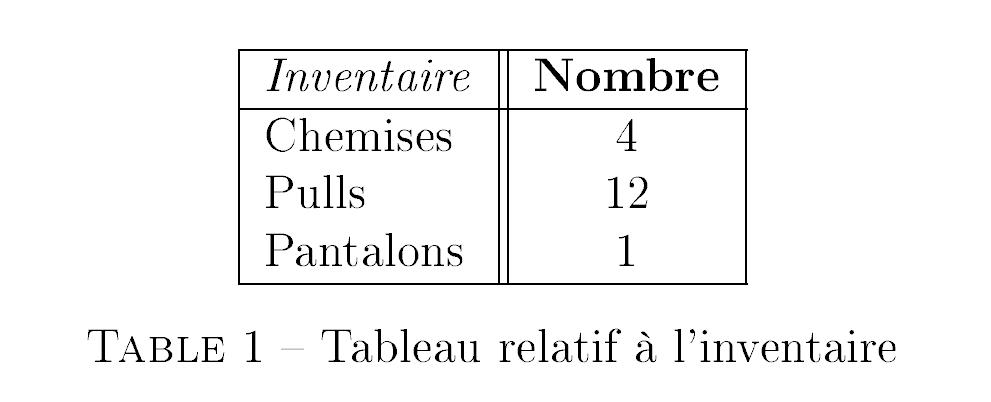
\includegraphics[width=0.6\textwidth]{table.jpg}}
\end{center}
\end{frame}
%-----------------------
\subsection{Les maths}
\begin{frame}[fragile]{L'environnement mathématique}
\framesubtitle{Inclure des formules dans le texte}
On peut ajouter une formule mathématique dans du texte entre deux symboles \textbf{\$}.

\begin{center}
\vspace{1cm}
	
	\Large
	\hspace{1cm} \verb|$x^{2n}$| \hspace{1cm} $\Rightarrow$ \hspace{1cm}  $x^{2n}$
	\medskip
	
	\hspace{1cm} \verb|$\sin(x)$| \hspace{1cm} $\Rightarrow$ \hspace{1cm}  $\sin(x)$
\end{center}
	
\end{frame}

\begin{frame}[fragile]{L'environnement mathématique}
\framesubtitle{Formules numérotées}

Un environnement équation est prévu pour des formules plus longues, elles seront automatiquement centrées et numérotées pour être référencées (équation~\ref{eq:pnorm})

\begin{equation}
\label{eq:pnorm}
p(x)=\frac{1}{\sigma \sqrt{2\pi}}\exp
		 \left(-\frac{(x-\mu)^2}{2\sigma^2}\right)
\end{equation}

\vspace{0.2cm}
\begin{center}
\begin{footnotesize}
	\begin{verbatim}
(équation~\ref{eq:pnorm})

\begin{equation}
\label{eq:pnorm}

p(x)=\frac{1}{\sigma \sqrt{2\pi}}\exp 
         \left(-\frac{(x-\mu)^2}{2\sigma^2}\right)

\end{equation}
\end{verbatim}

\end{footnotesize}
\end{center}
	
\end{frame}

%%%%%%%%%%%%%

\section{Références}

\subsection{Références des éléments du texte}
\begin{frame}
\frametitle{\insertsubsection}
\begin{itemize}
	\item Facile de faire référence à un numéro et la page d'une section et d'un environnement (\texttt{figure}, \texttt{equation}, \texttt{table}).\\
	\item On place une étiquette d'un côté (\texttt{\symbol{92}label\{mon\_label\}}) et on peut utiliser \texttt{\symbol{92}ref\{mon\_label\}} ou \texttt{\symbol{92}pageref\{mon\_label\}} voir \texttt{\symbol{92}vpageref\{mon\_label\}} du paquet \texttt{varioref} avec l'option \texttt{[french]} pour imprimer le numéro ou la page correspondante.\\
\end{itemize}
\label{ref} Exemple: nous sommes à la section \ref{ref}, page \pageref{ref}, \vpageref{ref}.\\
\vspace{.5cm}
$\Rightarrow$ \texttt{\symbol{92}label\{ref\} Exemple: nous sommes à la section \symbol{92}ref\{ref\}, page \symbol{92}pageref\{ref\}, \symbol{92}vpageref\{ref\}}.

\end{frame}

\subsection{Bibliographie}
\begin{frame}
\frametitle{\insertsubsection}
Deux possibilités pour maintenir une bibliographie:
\begin{itemize}
	\item Éditer une bibliographie à la main (s'il y a très peu de référence, voir exemple)
	\item Utiliser des fichiers \texttt{bib}.
	\begin{itemize}
		\item Disponible avec les revues scientifiques
		\item En utilisant le plugin \href{https://www.zotero.org/}{Zotero} pour récupérer les informations d'un \href{http://www.amazon.fr/LaTeX-HowTo-S\%C3\%A9bastien-Comb\%C3\%A9fis/dp/1446708314/ref=sr_1_5?ie=UTF8&qid=1363022579&sr=8-5}{site}
		\item Il faut "compiler" le fichier Bib\TeX{} puis "recompiler" le document.
	\end{itemize}
\end{itemize}
Puis il suffit d'utiliser dans son texte la commande \texttt{cite} avec l'étiquette de la source à référencer pour ajouter une référence à cette source et ajouter la source dans la bibliographie.
\end{frame}

\subsection{En vrac}
\begin{frame}
\frametitle{\insertsubsection}
Dans le même domaine, on peut parler des annexes (\texttt{\symbol{92}Appendix}), mais également des environnements \texttt{abstract}, \texttt{quotation}, etc.\\
\vspace{1cm}
Astuce sympa, on peut séparer un document en plusieurs petits fichiers et les inclure avec la commande \texttt{input} avec le nom du fichier en seul paramètre. Attention que seul le document principal (qui contient le \texttt{\symbol{92}begin\{document\}}) peut compiler!\\
\vspace{1cm}
Pour avoir un plus grand aperçu, n'hésitez pas à consulter le livre \LaTeX{} How To, les slides et exercices avancées disponibles sur notre site mais à regarder les nombreux boutons que comportent les éditeurs de texte dédiés à \LaTeX.
\end{frame}

\AtBeginSection[]{} %% stop TOC

\section{Exercices}
\begin{frame}
\frametitle{Exerçons-nous}
	\begin{itemize}
		\item<1-> Télécharger le document \textbf{exemple.pdf}
		\item<2-> Reproduire une structure similaire :
			\begin{itemize}
				\item page de titre
				\item table des matières
				\item liste, tableau, figure
				\item math en ligne, hors-ligne
				\item références
				\item \dots
			\end{itemize}
		\item<3-> Chercher de l'information :
			\begin{itemize}
				\item \url{http://en.wikibooks.org/wiki/LaTeX}
				\item \url{http://www.grappa.univ-lille3.fr/FAQ-LaTeX}
				\item Google est ton ami !
				\item Livres:
				\begin{itemize}
					\item \LaTeX HowTo par Sébastien Combéfis (EN/FR)
					\item Framabook \LaTeX
				\end{itemize}
			\end{itemize}
	\end{itemize}

\end{frame}


\end{document}
